%% This is file `elsarticle-template-1-num.tex',
%%
%% Copyright 2009 Elsevier Ltd
%%
%% This file is part of the 'Elsarticle Bundle'.
%% ---------------------------------------------
%%
%% It may be distributed under the conditions of the LaTeX Project Public
%% License, either version 1.2 of this license or (at your option) any
%% later version.  The latest version of this license is in
%%    http://www.latex-project.org/lppl.txt
%% and version 1.2 or later is part of all distributions of LaTeX
%% version 1999/12/01 or later.
%%
%% Template article for Elsevier's document class `elsarticle'
%% with numbered style bibliographic references
%%
%% $Id: elsarticle-template-1-num.tex 149 2009-10-08 05:01:15Z rishi $
%% $URL: http://lenova.river-valley.com/svn/elsbst/trunk/elsarticle-template-1-num.tex $
%%

% \documentclass[preprint,12pt]{elsarticle}


%% Use the option review to obtain double line spacing
%% \documentclass[preprint,review,12pt]{elsarticle}

%% Use the options 1p,twocolumn; 3p; 3p,twocolumn; 5p; or 5p,twocolumn
%% for a journal layout:

\documentclass[final,1p,times]{elsarticle}

%% \documentclass[final,1p,times,twocolumn]{elsarticle}
%% \documentclass[final,3p,times]{elsarticle}
%% \documentclass[final,3p,times,twocolumn]{elsarticle}
%% \documentclass[final,5p,times]{elsarticle}
%% \documentclass[final,5p,times,twocolumn]{elsarticle}

%% The graphicx package provides the includegraphics command.
\usepackage{graphicx}
%% The amssymb package provides various useful mathematical symbols
\usepackage{amssymb}
%% The amsthm package provides extended theorem environments
%% \usepackage{amsthm}

%% The lineno packages adds line numbers. Start line numbering with
%% \begin{linenumbers}, end it with \end{linenumbers}. Or switch it on
%% for the whole article with \linenumbers after \end{frontmatter}.
\usepackage{lineno}

\usepackage{xcolor,listings}
\usepackage[colorlinks,linkcolor=black,urlcolor=black]{hyperref}

%% natbib.sty is loaded by default. However, natbib options can be
%% provided with \biboptions{...} command. Following options are
%% valid:

%%   round  -  round parentheses are used (default)
%%   square -  square brackets are used   [option]
%%   curly  -  curly braces are used      {option}
%%   angle  -  angle brackets are used    <option>
%%   semicolon  -  multiple citations separated by semi-colon
%%   colon  - same as semicolon, an earlier confusion
%%   comma  -  separated by comma
%%   numbers-  selects numerical citations
%%   super  -  numerical citations as superscripts
%%   sort   -  sorts multiple citations according to order in ref. list
%%   sort&compress   -  like sort, but also compresses numerical citations
%%   compress - compresses without sorting
%%
%% \biboptions{comma,round}

% \biboptions{}

\journal{Database System Technology}

\begin{document}

\begin{frontmatter}

%% Title, authors and addresses

\title{Lab Project: OpenStreetMap}

%% use the tnoteref command within \title for footnotes;
%% use the tnotetext command for the associated footnote;
%% use the fnref command within \author or \address for footnotes;
%% use the fntext command for the associated footnote;
%% use the corref command within \author for corresponding author footnotes;
%% use the cortext command for the associated footnote;
%% use the ead command for the email address,
%% and the form \ead[url] for the home page:
%%
%% \title{Title\tnoteref{label1}}
%% \tnotetext[label1]{}
%% \author{Name\corref{cor1}\fnref{label2}}
%% \ead{email address}
%% \ead[url]{home page}
%% \fntext[label2]{}
%% \cortext[cor1]{}
%% \address{Address\fnref{label3}}
%% \fntext[label3]{}


%% use optional labels to link authors explicitly to addresses:
%% \author[label1,label2]{<author name>}
%% \address[label1]{<address>}
%% \address[label2]{<address>}

\author{Zhenfeng Shi}
\author{Hongru Zhu}
\author{Chang Zhou}

\address{jack.shi2013@gmail.com}

\begin{abstract}
%% Text of abstract

\end{abstract}

\begin{keyword}
OSM \sep Database
%% keywords here, in the form: keyword \sep keyword

%% MSC codes here, in the form: \MSC code \sep code
%% or \MSC[2008] code \sep code (2000 is the default)

\end{keyword}

\end{frontmatter}

%%
%% Start line numbering here if you want
%%
\linenumbers

%% main text
\section{Usage}
\subsection{Environment}
Python 3 + pymysql 
\subsection{Install}
Enter the root path of this project, run the following command in the shell:
\begin{verbatim}
python SZZ_install.py [-h] [-c host] [-u user] [-p passwd] [-n dbname] [-i input]

                     -c:  host connect, for instance 'localhost'
                     -u:  username for mysql, for instance 'root'
                     -p:  password for mysql, ignore this if no password
                     -n:  name for the new database
                     -i:  inputfile path, for instance '../shanghai_dump.osm'
\end{verbatim}
For instance,

\begin{verbatim}
python SZZ_install -c localhost -u root -n OSM -i data/shanghai_dump.osm
\end{verbatim}

\subsection{Queries}

\section{Database Design}

\subsection{XML Parsing}

\subsection{E-R Model}

\subsection{SQL For Table Creation}
\begin{verbatim}
CREATE TABLE ways(
          			wayID VARCHAR(12),
                    LineString LINESTRING,
                    name VARCHAR(100), INDEX(name),
                    isRoad VARCHAR(100),
                    otherInfo TEXT,
                    PRIMARY KEY(wayID)
                ) ENGINE=MyISAM
                
CREATE TABLE nodes(
                    nodeID VARCHAR(12),
                    version TINYINT(1), INDEX(version),
                    version BOOLEAN,
                    PRIMARY KEY(nodeID)
                ) ENGINE=MyISAM
                
CREATE TABLE POIs(
                    nodeID VARCHAR(12),
                    position POINT NOT NULL, SPATIAL INDEX(position),
                    planaxy POINT NOT NULL, SPATIAL INDEX(planaxy),
                    name VARCHAR(100), INDEX(name),
                    poitype VARCHAR(100), INDEX(poitype),
                    otherInfo TEXT,
                    PRIMARY KEY(nodeID)
                ) ENGINE=MyISAM
                
create table nonPOIs(
                    nodeID VARCHAR(12),
                    position POINT NOT NULL, SPATIAL INDEX(position),
                    planaxy POINT NOT NULL, SPATIAL INDEX(planaxy),
                    otherInfo TEXT,
                    PRIMARY KEY(nodeID)
                ) ENGINE=MyISAM
                
create table WayNode(
                     wayID VARCHAR(12), INDEX(wayID),
                     nodeID VARCHAR(12), INDEX(nodeID),
                     node_order INT(2),
                     FOREIGN KEY (nodeID) REFERENCES nodes(nodeID),
                     FOREIGN KEY (wayID) REFERENCES ways(wayID)
                ) ENGINE=MyISAM                
\end{verbatim}

\subsection{Data Insertion}
For the data we parsed from XML, we inserted them into corresponding fields of our created tables.

Notably, if we insert the data directly into the table, the insertion time complexity would be $O(log(N))$, where N is the entries already existed in the table, due to the index (primary key) building process.

Therefore, in order to speed up the insertion process, we disable all the keys before the insertion, and enable them after the insertion. This will ensure every row is inserted in time complexity $O(N)$.

The SQL code is as follows:

\begin{verbatim}
              LOCK TABLE `nodes`, `pois`, `nonpois` WRITE;
              ALTER TABLE `nodes` DISABLE KEYS;
              ALTER TABLE `pois` DISABLE KEYS;
              ALTER TABLE `nonpois` DISABLE KEYS;
              /*...insertion...*/
              ALTER TABLE `nodes` ENABLE KEYS;
              ALTER TABLE `pois` ENABLE KEYS;
              ALTER TABLE `nonpois` ENABLE KEYS;
              UNLOCK TABLES;
\end{verbatim}

The \textbf{LOCK TABLE} is to make sure no other users are writing at the same time.
\subsection{Index}
Besides index for primary keys, we built 8 indexes to accelerate the queries. Especially, in order to speed up the spatial queries, we applied Spatial Index in MySQL. For \emph{MyISAM} tables, Spatial Index creates an R-tree index. The key idea of the R-tree is to group nearby objects and represent them with their minimum bounding rectangle in the next higher level of the tree. For storage engines that support non-spatial indexing of spatial columns, the engine creates a B-tree index. A B-tree index on spatial values is useful for exact-value lookups, but not for range scans. In our cases, the R-tree is more suitable because required query 4, 5, 6 all include range scans.

\begin{figure}[thpb]
      \centering
      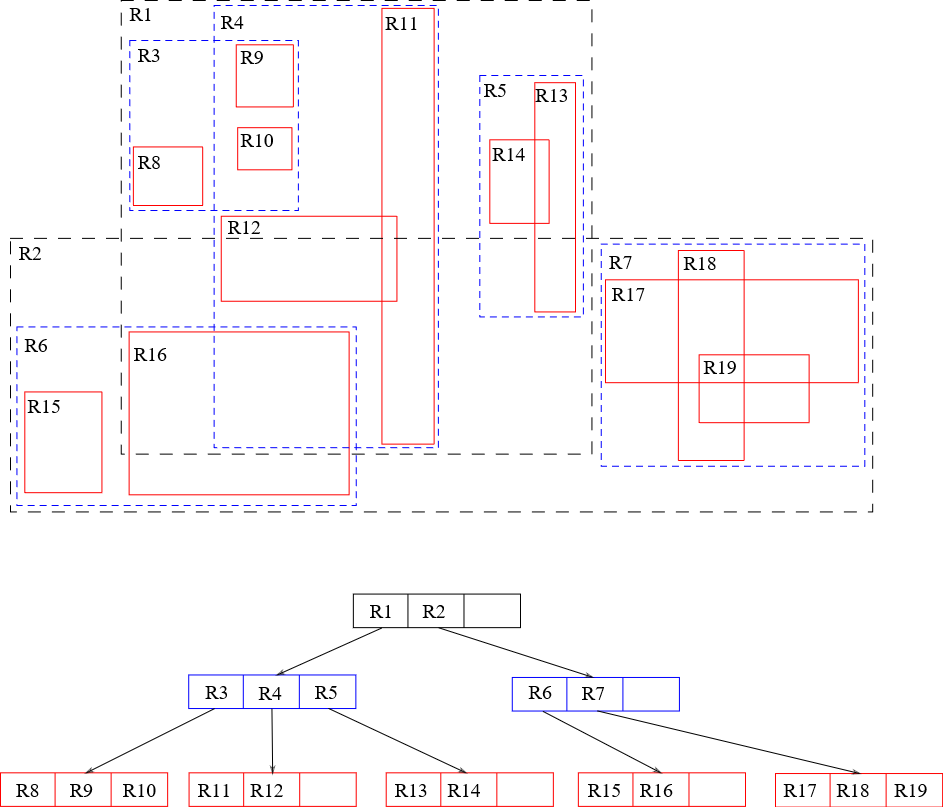
\includegraphics[width=3in]{R-tree.png}
      \caption{R-tree in 2 dimention}
      \label{fig:Rtree}
\end{figure}


\section{Point Mapping}
The longtitude and latitude are used as the absolute coordinates. However, when calculating the distance between two points of given longtitude and latitude, we have to take spherical properties into consideration.

For instance, the distance between $(30.4, 122.1)$ and $(30.4, 122.6)$ is $48.0073$ Km. The distance between $(32.4, 122.1)$ and $(32.4, 122.6)$ is $46.995$ Km. There would be a error about $1$ Km if we ignore the spherical properties of the Earth.

\subsection{Different Ways of Calculating Distances Between Two Given Coordinates}
\begin{enumerate}
\item[a)] Vincenty's formulae are two related iterative methods used in geodesy to calculate the distance between two points on the surface of a spheroid, developed by Thaddeus Vincenty (1975). They are based on the assumption that the figure of the Earth is an oblate spheroid, and hence are more accurate than methods that assume a spherical Earth.
For simplicity and focus on the course related work, here we only provide the link to the Vincenty’s paper without further explanation. 
(\url{http://www.ngs.noaa.gov/PUBS_LIB/inverse.pdf})

\item[b)] Another approach is to map latitude-longitude coordinates to plana coordinates and then calculate the distance in between. We used the definition of Miller’s cylindrical projection, which is more accurate near the equator. Further about the derivation please see the original paper. (\url{http://www.jstor.org/stable/210384})
\end{enumerate}

\subsection{Implementation}
We randomly sampled the start and the destination and got the distribution of the distance error derived using two methods. We concluded that the Vincenty distance, which is more accurate, was 0.66~1.15 times of the Miller distance. This is further explored in our Query 4 and Query 5 design.

\begin{figure}[thpb]
      \centering
      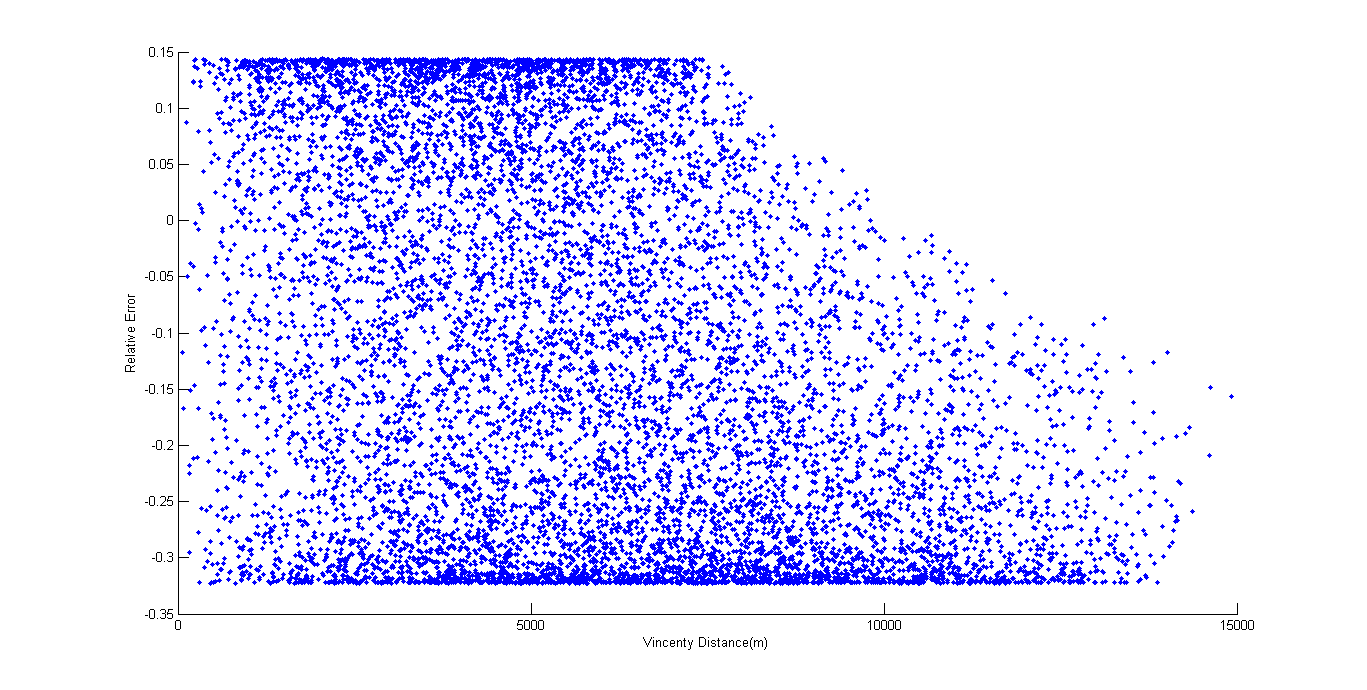
\includegraphics[width=14cm]{Vincenty.png}
      \caption{Relative error between miller distance and vincenty distance}
      \label{fig:Vincenty}
\end{figure}

\section{Solution to Required Queries}
\begin{enumerate}
  \item Give a node, return all ways taht contain it, and infer whether the node is an intersection of roads, i.e., a crossroad.
  \item Given a way, return all the nodes along the way.
  \item Search the name of the road and return information of those matched.
  \item Query the POIs within a radius of a given location (Longtitude-latitude coordinates).
  \item Find the closest road to a given GPS coordinate.
  \item Implement an API to return the XML in osm format defined in the wiki page, given a rectangular area bounding box (x1, y1, x2, y2) as parameters.
\end{enumerate}


\section{Extended Queries}


\section{Human Computer Interaction}




%% The Appendices part is started with the command \appendix;
%% appendix sections are then done as normal sections
%% \appendix

%% \section{}
%% \label{}

%% References
%%
%% Following citation commands can be used in the body text:
%% Usage of \cite is as follows:
%%   \cite{key}          ==>>  [#]
%%   \cite[chap. 2]{key} ==>>  [#, chap. 2]
%%   \citet{key}         ==>>  Author [#]

%% References with bibTeX database:

\bibliographystyle{model1-num-names}
\bibliography{sample.bib}

%% Authors are advised to submit their bibtex database files. They are
%% requested to list a bibtex style file in the manuscript if they do
%% not want to use model1-num-names.bst.

%% References without bibTeX database:

% \begin{thebibliography}{00}

%% \bibitem must have the following form:
%%   \bibitem{key}...
%%

% \bibitem{}

% \end{thebibliography}


\end{document}

%%
%% End of file `elsarticle-template-1-num.tex'.\documentclass[preprint,12pt]{elsarticle}
